\chapter{TINJAUAN PUSTAKA}

% Ubah konten-konten berikut sesuai dengan isi dari tinjauan pustaka
\section{Hasil penelitian/perancangan terdahulu}
Dalam penelitian ini, penulis merujuk pada beberapa studi sebelumnya yang relevan. Penelitian-penelitian tersebut memiliki hubungan dengan topik yang sedang diteliti, sehingga dapat digunakan sebagai dasar untuk penelitian ini.

\section{Hasil Penelitian/Perancangan Terdahulu}



\subsection{\emph{Intelligent Identification Method of Transformer Overheat Fault in Distribution Substation Based on Deep Learning Algorithm and Infrared Temperature Measurement Technology}}
Penelitian oleh Kui Liu et al. (2023) membahas tentang metode identifikasi cerdas untuk mendeteksi kegagalan panas berlebih pada transformator di gardu distribusi. Metode ini menggabungkan teknologi pengukuran suhu inframerah dengan algoritma \emph{deep learning}. Dalam studi ini, termometer inframerah dipilih sebagai alat utama untuk mengidentifikasi kondisi overheating pada transformator.

Hasil eksperimen menunjukkan bahwa metode ini memiliki kinerja pengenalan yang baik, keandalan yang tinggi, serta nilai aplikasi yang signifikan, yang berkontribusi dalam mengurangi risiko operasional pada transformator di gardu distribusi. Sistem ini beroperasi dengan menangkap radiasi inframerah dari transformator menggunakan kamera termal inframerah, yang kemudian dihubungkan ke server dan komputer melalui jaringan LAN/WAN. Data yang ditangkap oleh kamera inframerah diproses menggunakan algoritma algoritma \emph{deep learning} untuk menganalisis potensi overheating pada transformator. Penelitian ini memiliki kesamaan dengan topik kami, yang juga menggunakan kamera termal dan algoritma pembelajaran mesin untuk mendeteksi kondisi panas berlebih pada transformator \cite{KuiLiau2023}.

\subsection{\emph{Autonomous Thermal Vision Robotic System for Victims Recognition in Search and Rescue Missions}}
Penelitian oleh Cruz Ulloa mengembangkan robot berkaki empat (\emph{quadruped}) yang dilengkapi dengan kamera termal dan \emph{Convolutional neural network (CNN)} untuk mendeteksi korban dalam misi pencarian di lingkungan pasca-bencana. Penelitian ini berhasil mencapai akurasi lebih dari 90\% dalam kondisi lingkungan sulit, seperti minim cahaya dan puing-puing. Robot ini mampu bergerak secara otonom dan mendeteksi korban dengan cepat, sehingga dapat membantu tim pencarian dalam menemukan korban yang terperangkap di lokasi bencana\cite{Cruz2021}. Penelitian tersebut memiliki kesamaan dengan topik kami yang sama-sama menggunan \emph{quadruped} dan kamera termal. 

\begin{figure} [H] \centering
  % Nama dari file gambar yang diinputkan
  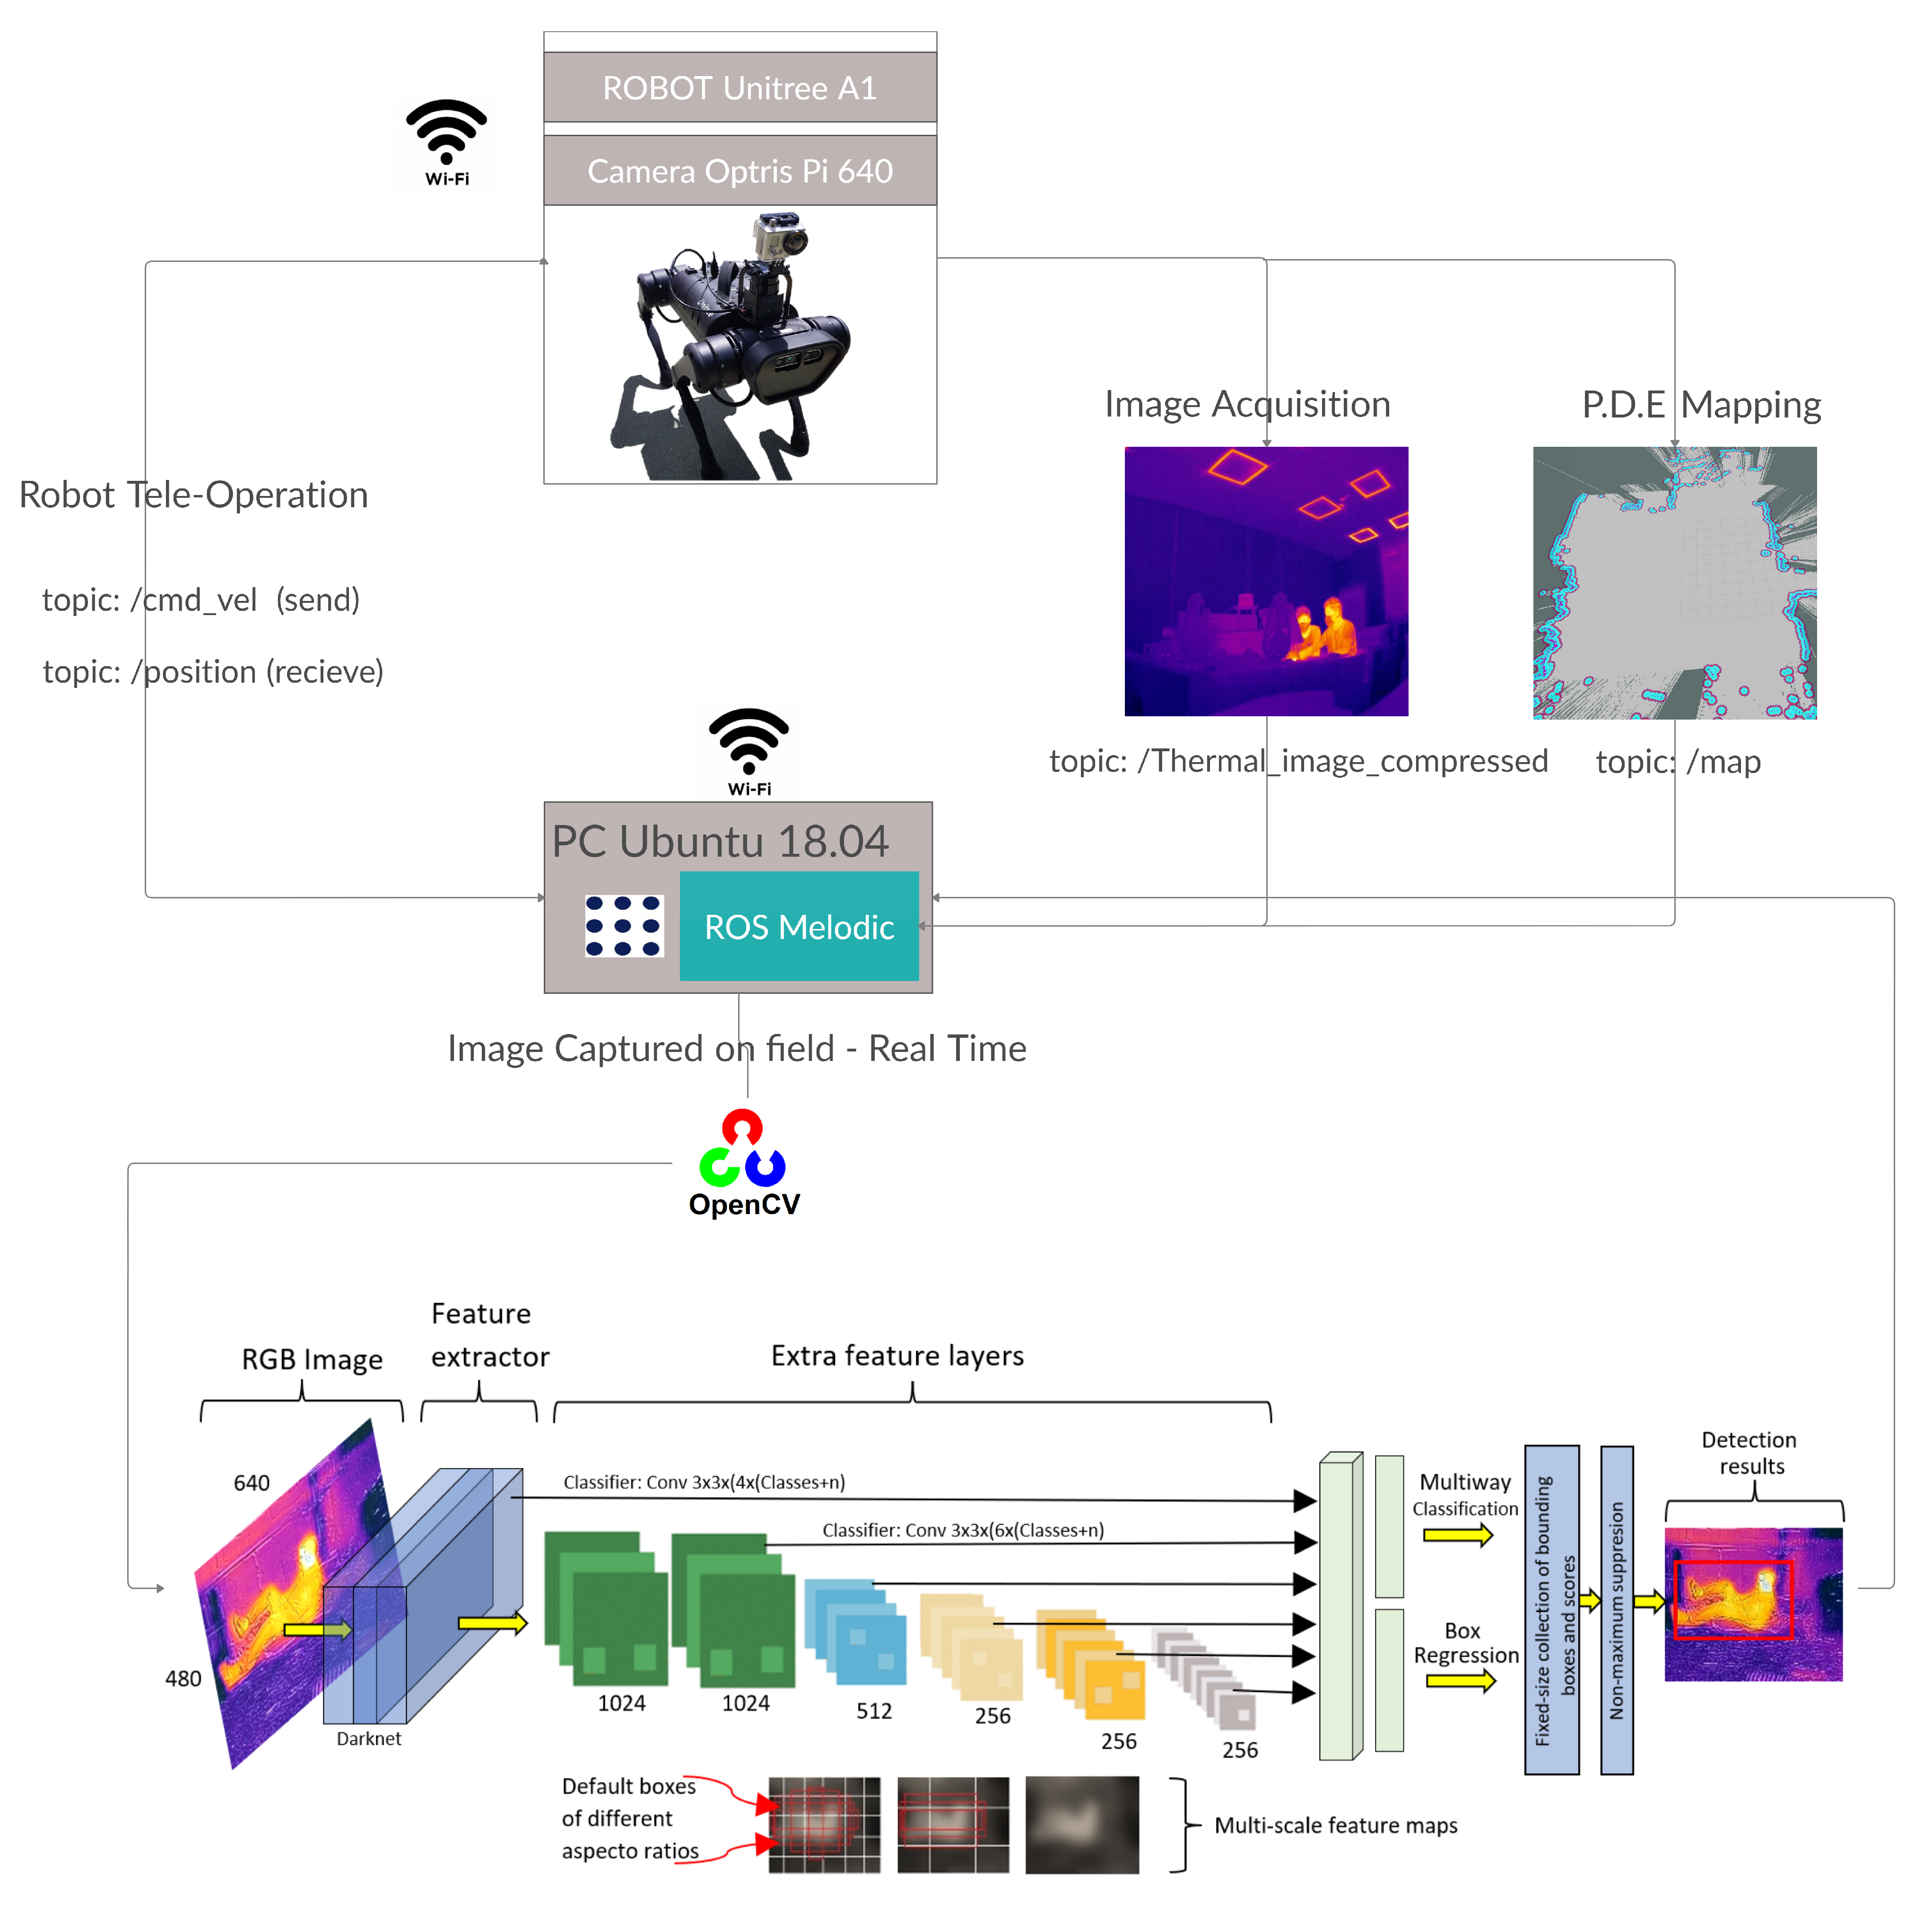
\includegraphics[scale=0.1]{gambar/unitreea1.png}
  % Keterangan gamßbar yang diinputkan
  \caption{\emph{Quadruped robot} dengan kamera termal untuk deteksi korban}
  % Label referensi dari gambar yang diinputkan
  \label{fig:Quadruped  dengan kamera termal untuk deteksi korban}
\end{figure}

\newpage